\clearpage
\appendix
\section*{APPENDIX A}
\addcontentsline{toc}{section}{\numberline{} APPENDIX A}
\setcounter{section}{8}
\subsection{Signal Processsing}
In signal processing, a window function (also known as an apodization function or tapering
function) is a mathematical function that is zero-valued outside of some chosen interval. For
instance, a function that is constant inside the interval and zero elsewhere is called
a rectangular window, which describes the shape of its graphical representation. When
another function or waveform/data-sequence is multiplied by a window function, the product
is also zero-valued outside the interval: all that is left is the part where they overlap, the
"view through the window".\\
\\
Applications of window functions include spectral analysis, filter design, and beam forming.
In typical applications, the window functions used are non-negative smooth "bell-shaped"
curves, though rectangle, triangle, and other functions can be used.
A more general definition of window functions does not require them to be identically zero
outside an interval, as long as the product of the window multiplied by its argument is square
integral, and, more specifically, that the function goes sufficiently rapidly toward zero.
One of the major applications of window functions includes the design of finite impulse
response filters and the spectral analysis.\\
\\
\subsection{Spectral Analysis}
The Fourier transform of the function cos ωt is zero, except at frequency ±ω. However, many
other functions and waveforms do not have convenient closed form transforms. Alternatively,
one might be interested in their spectral content only during a certain time period.
In either case, the Fourier transform (or something similar) can be applied on one or more
finite intervals of the waveform. In general, the transform is applied to the product of the
waveform and a window function. Any window (including rectangular) affects the spectral
estimate computed by this method.\\

\subsection{Windowing}
Windowing of a simple waveform like cos ωt causes its Fourier transform to develop non-
zero values (commonly called spectral leakage) at frequencies other than ω. The leakage
tends to be worst (highest) near ω and least at frequencies farthest from ω.
If the waveform under analysis comprises two sinusoids of different frequencies, leakage can
interfere with the ability to distinguish them spectrally. If their frequencies are dissimilar and
one component is weaker, then leakage from the larger component can obscure the weaker
one‟s presence. But if the frequencies are similar, leakage can render them irresolvable even
when the sinusoids are of equal strength.\\
\\
The rectangular window has excellent resolution characteristics for sinusoids of comparable
strength, but it is a poor choice for sinusoids of disparate amplitudes. This characteristic is
sometimes described as low-dynamic-range.\\
\\
At the other extreme of dynamic range are the windows with the poorest resolution. These
high-dynamic-range low-resolution windows are also poorest in terms of sensitivity; this is, if
the input waveform contains random noise close to the frequency of a sinusoid, the response
to noise, compared to the sinusoid, will be higher than with a higher-resolution window. In
other words, the ability to find weak sinusoids amidst the noise is diminished by a high-
dynamic-range window. High-dynamic-range windows are probably most often justified in
wideband applications, where the spectrum being analyzed is expected to contain many
different components of various amplitudes.\\
\\
In between the extremes are moderate windows, such as Hamming and Hann. They are
commonly used in narrowband applications, such as the spectrum of a telephone channel. In
summary, spectral analysis involves a tradeoff between resolving comparable strength
components with similar frequencies and resolving disparate strength components with
dissimilar frequencies. That tradeoff occurs when the window function is chosen.

\subsection{Filter Bank}
In signal processing, a filter bank is an array of band-pass filters that separates the input
signal into multiple components, each one carrying a single frequency sub-band of the
original signal. One application of a filter bank is a graphic equalizer, which can attenuate the
components differently and recombine them into a modified version of the original signal.
The process of decomposition performed by the filter bank is called analysis (meaning
analysis of the signal in terms of its components in each sub-band); the output of analysis is
referred to as a sub band signal with as many sub bands as there are filters in the filter bank.
The reconstruction process is called synthesis, meaning reconstitution of a complete signal
resulting from the filtering process.\\
\\
In digital signal processing, the term filter bank is also commonly applied to a bank of
receivers. The difference is that receivers also down-convert the sub bands to a low center
frequency that can be re-sampled at a reduced rate. The same result can sometimes be
achieved by under sampling the band pass sub bands.\\
\\
Another application of filter banks is signal compression, when some frequencies are more
important than others. After decomposition, the important frequencies can be coded with a
fine resolution. Small differences at these frequencies are significant and a coding scheme
that preserves these differences must be used. On the other hand, less important frequencies
do not have to be exact. A coarser coding scheme can be used, even though some of the finer
(but less important) details will be lost in the coding.\\
\\
The vocoder uses a filter bank to determine the amplitude information of the sub bands of a
modulator signal (such as a voice) and uses them to control the amplitude of the sub bands of
a carrier signal (such as the output of a guitar or synthesizer), thus imposing the dynamic
characteristics of the modulator on the carrier.\\

\newpage
\subsection{GUI}
\begin{figure}[h!]
        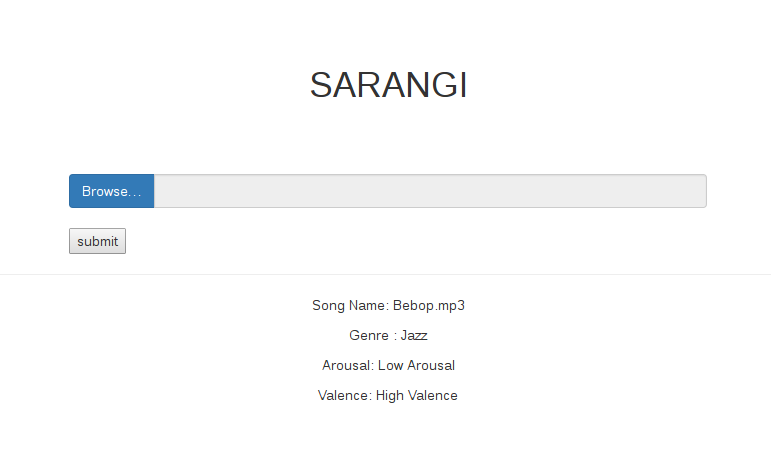
\includegraphics[width=150mm]{resources/gui}
        \caption{Graphics user interface}
\end{figure}
